\documentclass{ximera}
      
\title{Limits}
      
\begin{document}
      
\begin{abstract}
      
Limits.      
\end{abstract}
      
\maketitle
Consider the graph of $y=f(x)$.
$$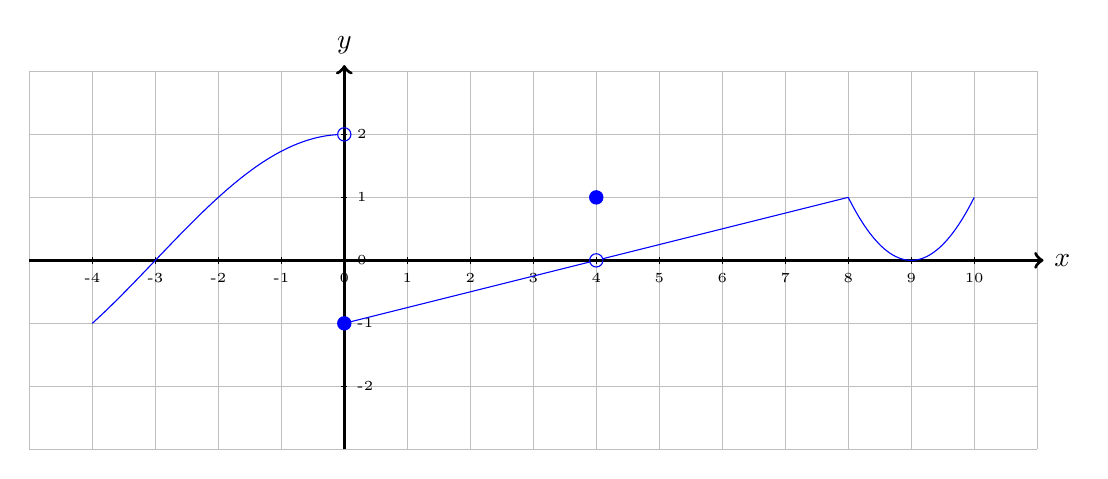
\begin{tikzpicture}[scale=.8][domain=-5:11]
    \draw[gray!50, thin, step=1] (-5,-3) grid (11,3);
    \draw[very thick,->] (-5,0) -- (11.1,0) node[right] {$x$};
    \draw[very thick,->] (0,-3) -- (0,3.1) node[above] {$y$};

    \foreach \x in {-4,...,10} \draw (\x,0.05) -- (\x,-0.05) node[below] {\tiny\x};
    \foreach \y in {-2,...,2} \draw (-0.05,\y) -- (0.05,\y) node[right] {\tiny\y};

    \draw[blue] (0,2) circle (3pt);
    \draw[fill, blue] (0,-1) circle (3pt);
    \draw[blue] (4,0) circle (3pt);
    \draw[fill, blue] (4,1) circle (3pt);


  \draw[scale=1,domain=-4:-.1,smooth,variable=\x,blue] plot ({\x},{2*cos(3.141595*\x r/6)});
  \draw[scale=1,domain=0:3.9,smooth,variable=\x,blue] plot ({\x},{\x/4-1});
  \draw[scale=1,domain=4.1:8,smooth,variable=\x,blue] plot ({\x},{\x/4-1});
  \draw[scale=1,domain=8:10,smooth,variable=\x,blue] plot ({\x},{(\x-9)*(\x-9)});


\end{tikzpicture}$$
 
 \begin{problem}
 Identify the following, write DNE if the value does not exist.
 
 \begin{enumerate}
\item $\displaystyle\lim_{x\to 0^-} f(x)=\answer{2}$
\item $\displaystyle\lim_{x\to 0^+} f(x)=\answer{-1}$
\item $\displaystyle\lim_{x\to 0} f(x)=\answer{DNE}$
\item $f(0)=\answer{-1}$
\item $\displaystyle\lim_{x\to 4^-} f(x)=\answer{0}$
\item $\displaystyle\lim_{x\to 4^+} f(x)=\answer{0}$
\item $\displaystyle\lim_{x\to 4} f(x)=\answer{0}$
\item $f(4)=\answer{1}$
\item $\displaystyle\lim_{x\to 8^-} f(x)=\answer{1}$
\item $\displaystyle\lim_{x\to 8^+} f(x)=\answer{1}$
\item $\displaystyle\lim_{x\to 8} f(x)=\answer{1}$
\item $f(8)=\answer{1}$


\end{enumerate}

 
 
 \end{problem}
 
 \begin{problem}
 For which of the following values of $x$ is $f$ continuous?
 
 \begin{multipleChoice}
 \choice{x=0}
 \choice{x=4}
 \choice[correct]{x=8}
 \end{multipleChoice}
 
 
 \end{problem}
      






\end{document}
